%% BEAMER THEME FLIP 2012: Main tex file for compiling
%$ Compile this file. 
%%
%% Copyright 2012 by Flip Tanedo
%% This file may be distributed and/or modified
%% 	1. under the LaTeX Project Public License and/or
%% 	2. under the GNU Public License.
%% 
%% If you e-mail Flip (pt267@cornell.edu) to say that you
%% like this style file, then it would make him smile.

%% Please see notes.txt for comments on Beamer Theme Flip 2013
%% By default, this template is meant to be run with XeLaTeX (for fonts)
%% To run in PDFLaTeX, remove fontspec and any font commands

%% Discussion of Beamer vs XeLaTeX vs LuaLaTeX
%% http://tex.stackexchange.com/questions/29497/xelatex-preventing-beamer-from-using-different-backgrounds



\documentclass[12pt]{beamer}
\usetheme[
	bullet=circle,		% Other option: square
	bigpagenumber,		% circled page number on lower right
	topline=true,			% colored bar at the top of the frame 
	shadow=false,			% Shading for beamer blocks
	watermark=BG_lower,	% png file for the watermark
	]{Flip}


\newcommand{\titleimage}{title}			% Custom title 
\newcommand{\tanedo}{tanedolight}		% Custom author name
\newcommand{\CMSSMDM}{CMSSMDMlight.png}	% light background plot


%%%%%%%%%%
% FONTS %
%%%%%%%%%%

%% Default font: lmodern, doesn't require fontspec % solves some default warnings
\usepackage[T1]{fontenc}
\usepackage{lmodern}			
%\usepackage{sfmath}		% Sans Serif Math, off by default

%% Protects fonts from Beamer screwing with them
%% http://tex.stackexchange.com/questions/10488/force-computer-modern-in-math-mode
\usefonttheme{professionalfonts}


%% XeLaTeX fonts: (comment out if you don't use XeLaTeX)

%% For advanced fonts: access local OS X fonts
\usepackage[no-math]{fontspec}		
%% This template uses typical OS X and Adobe fonts
\defaultfontfeatures{Mapping=tex-text}	% This seems to be important for mapping glyphs properly

\setmainfont{GillSans}			% Beamer ignores "main font" in favor of sans font
\setsansfont{GillSans}			% This is the font that beamer will use by default
% \setmainfont{Gill Sans Light}		% Prettier, but harder to read

\setbeamerfont{title}{family=\fontspec{GillSans}}


\newcommand{\handwriting}{\fontspec{augie}} % From Emerald City, free font
% \newcommand{\handwriting}{}	% If you prefer no special handwriting font or don't have augie

%% Gill Sans doesn't look very nice when boldfaced
%% This is a hack to use Helvetica instead
%% Usage: \textbf{\forbold some stuff}
\newcommand{\forbold}{\fontspec{Helvetica}}
% \newcommand{\forbold}{} % if you want no special boldface



%%%%%%%%%%%%%%%%%%%%%%%%
% Usual LaTeX Packages %
%%%%%%%%%%%%%%%%%%%%%%%%

\usepackage{amsmath}
\usepackage{amsfonts}
\usepackage{amssymb}
\usepackage{graphicx}
\usepackage{mathrsfs} 			% For Weinberg-esque letters
\usepackage{cancel}				% For "SUSY-breaking" symbol
\usepackage{slashed}            % for slashed characters in math mode
\usepackage{bbm}                % for \mathbbm{1} (unit matrix)
\usepackage{amsthm}				% For theorem environment
\usepackage{multirow}			% For multi row cells in table
\usepackage{arydshln} 			% For dashed lines in arrays and tables
\usepackage{tikzfeynman}		% For Feynman diagrams
% \usepackage{subfig}           % for sub figures
% \usepackage{young}			% For Young Tableaux
% \usepackage{xspace}			% For spacing after commands
% \usepackage{wrapfig}			% for Text wrap around figures
% \usepackage{framed}
\usepackage{ulem}
\usepackage{anyfontsize}


\graphicspath{{images/}}	% Put all images in this directory. Avoids clutter.


\usetikzlibrary{backgrounds}
\usetikzlibrary{mindmap,trees}	% For mind map
% http://www.texample.net/tikz/examples/computer-science-mindmap/


% SOME COMMANDS THAT I FIND HANDY
% \renewcommand{\tilde}{\widetilde} % dinky tildes look silly, dosn't work with fontspec
\newcommand{\comment}[1]{\textcolor{comment}{\footnotesize{#1}\normalsize}} % comment mild
\newcommand{\Comment}[1]{\textcolor{Comment}{\footnotesize{#1}\normalsize}} % comment bold
\newcommand{\COMMENT}[1]{\textcolor{COMMENT}{\footnotesize{#1}\normalsize}} % comment crazy bold
\newcommand{\Alert}[1]{\textcolor{Alert}{#1}} % louder alert
\newcommand{\ALERT}[1]{\textcolor{ALERT}{#1}} % loudest alert
%% "\alert" is already a beamer pre-defined



\author{Dang Fan, Wang Shuhao, Ding Peng}
\title[AR on CTM]{An Article Recommendation System Based on Collaborative Topic Modeling}
\institute{Tsinghua University}
\date{June 4, 2012}



\begin{document}

%%%%%%%%%%%%%%%%%%%%%%%%
% Additional  settings %
%%%%%%%%%%%%%%%%%%%%%%%%

%% To use external nodes; http://www.texample.net/tikz/examples/beamer-arrows/
\tikzstyle{every picture}+=[remember picture]


%%%%%%%%%%%%%%%%%%%%%%%%
% Actual content below %
%%%%%%%%%%%%%%%%%%%%%%%%

%% It's much nicer to have all the content in a separate file
% DO NOT COMPILE THIS FILE DIRECTLY!
% This is included by the the driver file (FlipBeamerTemplate.tex).

{ %% This is a total kludge for a fancy title page background
\setbeamertemplate{sidebar right}{\llap{
\includegraphics[width=\paperwidth,height=\paperheight]{BG_upper}}}
\begin{frame}[c]%{\phantom{title page}} 
% The \phantom{title page} is a kludge to get the red bar on top
% \titlepage
\begin{center}
	% \includegraphics[width=7cm]{WarpedPenguinsReturn}

	\begin{tikzpicture}%[show background grid] %% Use grid for positioning, then turn off
		\node[inner sep=0pt,above right] (title.png) 
			{ \includegraphics[width=10cm]{\titleimage} };
		% \node (title) at (1.5,1.5) {};
	\end{tikzpicture}
	\quad

	% \includegraphics[width=7cm]{\titleimage} 
	
	\vspace{2em}
	{\fontspec{augie}Dang Fan, Wang Shuhao, Ding Peng}
	\vspace{.5em}
	
	
\includegraphics[height=1.5cm]{THU}\\

	\textcolor{normal text.fg!50!Comment}{\sout{June 4}, 2012}
	% \textcolor{Comment}{ \;($\pi$ day)}\\
	% \Comment{4 February 2011}
\end{center}
\end{frame}
}



\begin{frame}[c]{\fontspec{Marker Felt}Overview}
	\Large
	\begin{itemize}
		\item Modeling
		\item Implementation
		\item Characteristics and performance
	\end{itemize}
	\normalsize
\end{frame}

\begin{frame}[c]{\fontspec{Marker Felt}Modeling}{Recommendations tasks}
	\begin{columns}[t]
	\begin{column}[T]{5cm}
		\begin{exampleblock}{Collaborative Filtering}
			\begin{itemize}
				\item User $i$: $u_i \in \mathbb{R}^K$
				\item Item $j$: $v_j \in \mathbb{R}^K$
				\item $\hat r_{ij} = u_i^Tv_j$
			\end{itemize}
		\end{exampleblock}
		\uncover<2->{
		\begin{exampleblock}{Probabilistic Matrix Factorization}
			\begin{itemize}
				\item $u_i \sim \mathcal{N}(0,\lambda_u^{-1}I_K)$
				\item $v_j \sim \mathcal{N}(0,\lambda_v^{-1}I_K)$
				\item $r_{ij} \sim \mathcal{N}(u_i^Tv_j,c_{ij}^{-1})$
			\end{itemize}
		\end{exampleblock}
		}
	\end{column}
	\begin{column}[T]{5.5cm}
		\uncover<3->{
		\begin{exampleblock}{Probabilistic Topic Models}
		    Latent Dirichlet Allocation
		    \begin{itemize}
		    	\item $K$ topics $\beta=\beta_{1:K}$
		    	\item For each article $w_j$
		    	\begin{enumerate}
		    		\item Topic distribution $\theta_j \sim$ Dirichlet($\alpha$)
		    		\item For each word $n$
		    		\begin{itemize}
		    			\item Topic $z_{jn}\sim$ Multinomial($\theta_j$)
		    			\item Word $w_{jn}\sim$ Multinomial($\beta_{z_{jn}}$)
		    		\end{itemize}
		    	\end{enumerate}
		    \end{itemize}
		\end{exampleblock}
		}
	\end{column}
	\end{columns}
\end{frame}

\begin{frame}[c]{\fontspec{Marker Felt}Modeling}{A hybrid approach}
	Collaborative Topic Regression
	\begin{enumerate}
		\item For each user $i$, $u_i \sim \mathcal{N}(0,\lambda_u^{-1}I_K)$
		\item For each item $j$,
			\begin{enumerate}[a)]
				\item Topic distribution $\theta_j \sim$ Dirichlet($\alpha$)
				\item Item latent offset $\epsilon_j \sim \mathcal{N}(0,\lambda_v^{-1}I_K)$\\
				$v_j=\epsilon_j+\theta_j$
				\item For each word $w_{jn}$,
					\begin{enumerate}[i.]
		    			\item Topic $z_{jn}\sim$ Multinomial($\theta_j$)
		    			\item Word $w_{jn}\sim$ Multinomial($\beta_{z_{jn}}$)
		    		\end{enumerate}
			\end{enumerate}
		\item For each user-item pair $(i,j)$, $r_{ij} \sim \mathcal{N}(u_i^Tv_j,c_{ij}^{-1})$
	\end{enumerate}
\end{frame}

\begin{frame}[c]{\fontspec{Marker Felt}Implementation}{The framework}
	\begin{center}
	\tikz[scale=0.7,transform shape,baseline=-2.5ex]\node[fill=charcoal!50!crimsonred, anchor=north, rounded corners, line width=.2ex] (a) 
	{
		\textcolor{white}{\large Preprocessor}
	};
	\quad
	\tikz[scale=0.7,transform shape,baseline=-2.5ex]\node[fill=COMMENT, anchor=north, rounded corners, line width=.2ex] (a) 
	{
		\textcolor{white}{\large LDA}
	};
	\quad
	\tikz[scale=0.7,transform shape,baseline=-2.5ex]\node[fill=jeans!50!black, anchor=north, rounded corners, line width=.2ex] (a) 
	{
		\textcolor{white}{\large CTR}
	};
	\end{center}

	\begin{center}
		\begin{tikzpicture}[scale=0.8,transform shape]%[mindmap, concept color=Alert, text=white, scale=0.7,transform shape]
			\Huge
			\begin{scope}[mindmap, concept color=Alert, text=white, scale=0.8,transform shape]
			\tikzstyle{level 1 concept}+=[sibling angle=120]
			\tikzstyle{level 2 concept}+=[sibling angle=45]
			
			\tikzstyle{root concept}+=[minimum size=1.5cm, text width=1cm] 
			
			\node[concept] (gf) {Article\\Recommendation System}
				[clockwise from = 90]
				child[concept color=charcoal!50!crimsonred]{node[concept] (mixing) {Preprocess}
					[clockwise from = 15]
					child[concept color=charcoal!50!crimsonred]{node[concept] (scalar) {Prune\\vocabulary TF-IDF}
						[clockwise from = 15]
						child[concept color=charcoal!50!crimsonred]{node[concept] (wvtool) {WVTool}}
					}
					child[concept color=charcoal!50!crimsonred]{node[concept] (kinetic) {Optimised\\vectors}}
				}
				child[concept color=COMMENT]{node[concept] (anomaly) {Latent Dirichlet Allocation}
				}
				child[concept color=jeans!50!black]{node[concept] (breaking) {Collaborative Topic Regression}
				}
			;
			\end{scope}
			%%
			\normalsize
			\node[draw, color=Alert, anchor=east, rounded corners, line width=.2ex] at (-3,1.5) {output};
			\node[draw, color=COMMENT!50!jeans, anchor=north, rounded corners, line width=.2ex] at (0,-2.5) {$\beta, \theta$ matrices};
			\node[draw, color=ALERT, anchor=west, rounded corners, line width=.2ex] at (2.5,1) {term counts};
		\end{tikzpicture}
	\end{center}
\end{frame}

\begin{frame}[c]{\fontspec{Marker Felt}Implementation}
	\begin{exampleblock}{Implementation of LDA}
		Expectation-Maximization Algorithm
		\begin{itemize}
			\item \textbf{E Step}: Calculate the expected value of the log likelihood function
			\item \textbf{M Step}: Find the parameter that maximizes this quantity
		\end{itemize}

		An open-source Java project \href{http://www.arbylon.net/projects/}{\texttt{lda-j}} can be found on the Internet.
	\end{exampleblock}
\end{frame}

\begin{frame}[c]{\fontspec{Marker Felt}Implementation}
	\begin{exampleblock}{Implementation of CTR}
		EM-style algorithm

		$$\mathcal{L}=-\frac{\lambda_u}{2}\Sigma_iu_i^Tu_i-\frac{\lambda_v}{2}\Sigma_j(v_j-\theta_j)^T(v_j-\theta_j)$$
		$$+\Sigma_j\Sigma_n\log(\Sigma_k\theta_{jk}\beta_{k,w_{jn}})-\Sigma_{i,j}\frac{c_{ij}}{2}(r_{ij}-u_i^Tv_j)^2$$
	\end{exampleblock}
\end{frame}

\begin{frame}[c]{\fontspec{Marker Felt}Characteristics}
	\Large
	\begin{itemize}
		\item A hybrid approach
		\item \Alert{Good} performance
	\end{itemize}
	\normalsize
\end{frame}

\begin{frame}[c]{\fontspec{Marker Felt}Performance}
	\begin{tabular}{lcll}\hline 
	\textbf{K(Topics)} & \textbf{Accuracy(of 5)} & \textbf{AP@5} & \textbf{Running Time} \\
	\hline
25 & 2.9831 & 0.7435 & 40min\\
50 & 3.4597 & 0.8296 & 54min\\
75 & 3.6293 & 0.8545 & 1.8h\\
100 & 3.7348 & 0.8717 & 3.5h\\
125 & 3.7709 & 0.8794 & 4.3h\\
150 & 3.8080 & 0.8812 & 7.0h\\
175 & 3.8258 & 0.8873 & 9.8h\\
200 & 3.8427 & 0.8881 & 13.2h\\
	\hline 
	\end{tabular}
\end{frame}


\begin{frame}[c]{\fontspec{Marker Felt}Performance}{Accuracy}
	\begin{figure}
		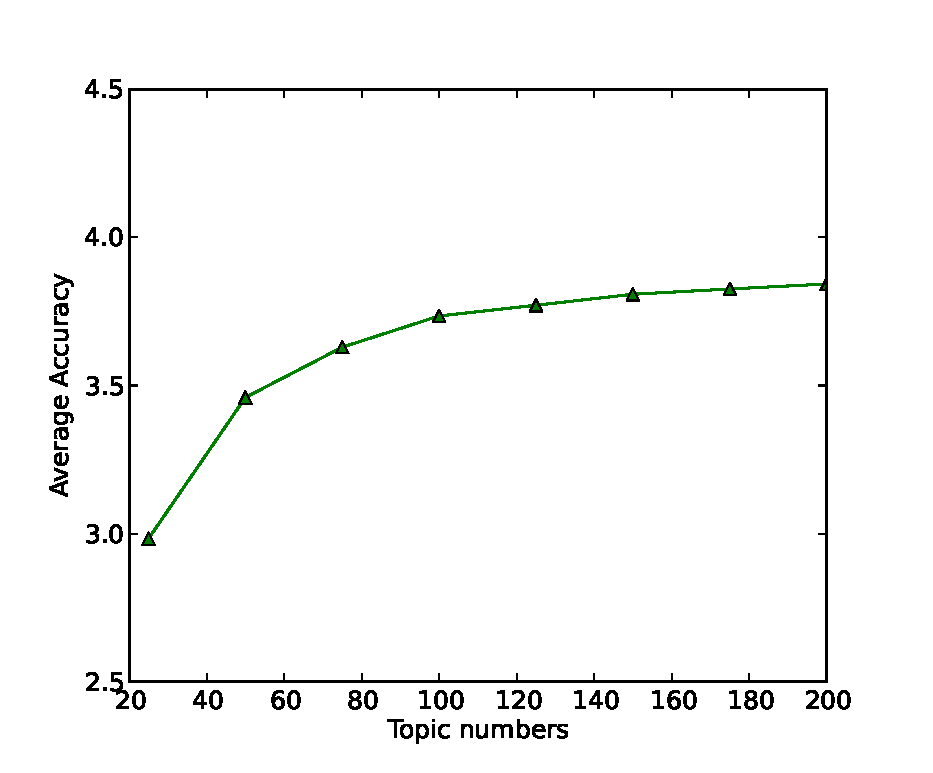
\includegraphics[width=9cm]{acc.eps}
	\end{figure}
\end{frame}

\begin{frame}[c]{\fontspec{Marker Felt}Performance}{AP@5}
	\begin{figure}
		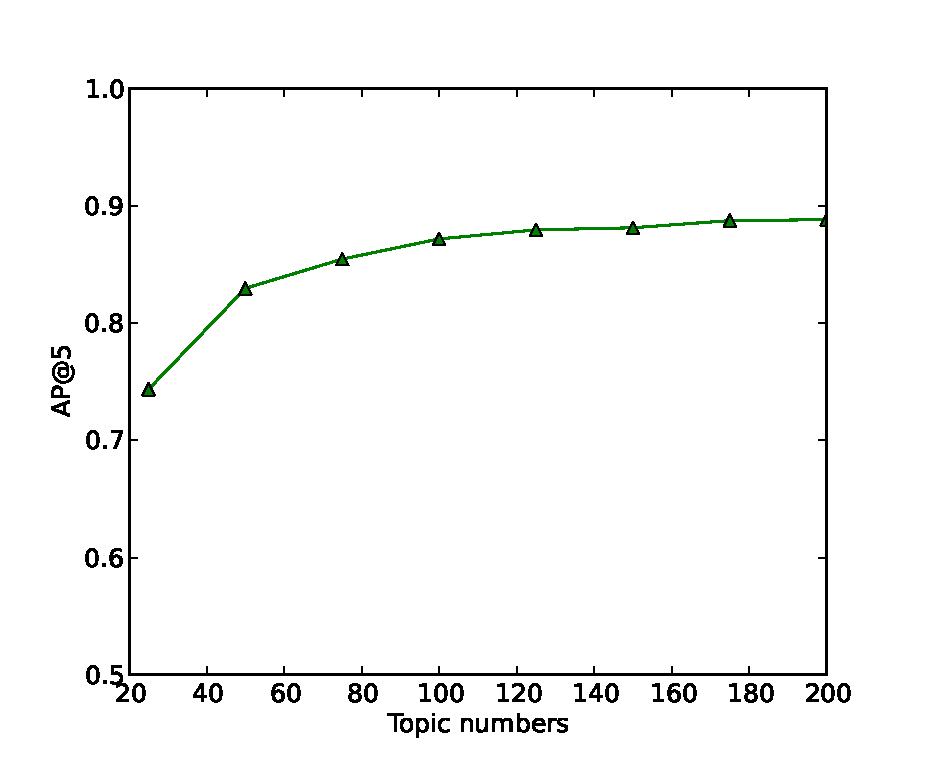
\includegraphics[width=9cm]{ap.eps}
	\end{figure}
\end{frame}

\begin{frame}[c]{\fontspec{Marker Felt}Performance}{Running Time}
	\begin{figure}
		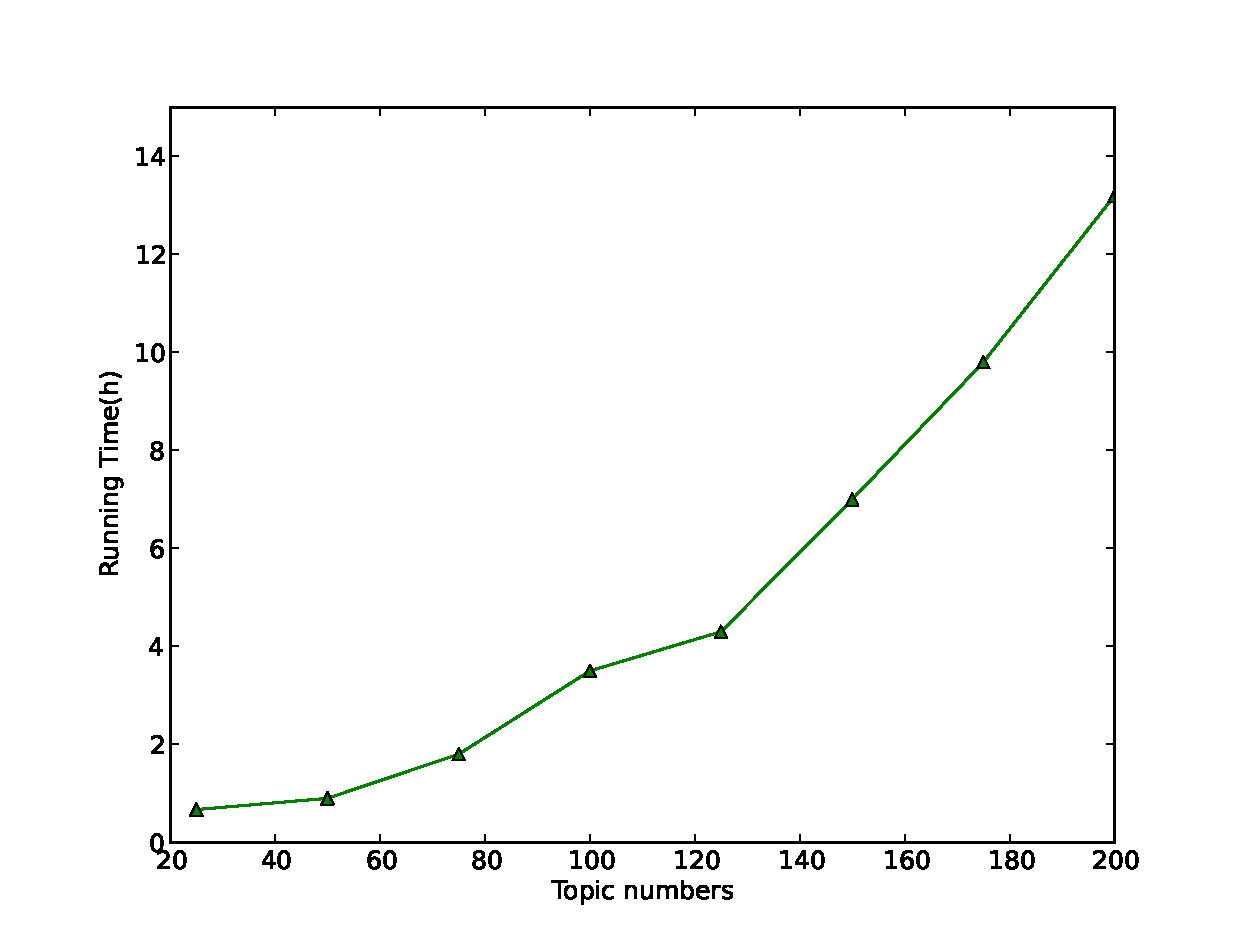
\includegraphics[width=10cm]{time.eps}
	\end{figure}
\end{frame}

\addtocounter{framenumber}{-1}
\begin{frame}[c]{}
	\begin{center}
	\ALERT{\fontsize{50}{60}\selectfont\fontspec{Marker Felt}Thanks}
	\end{center}
\end{frame}



% \begin{frame}{test}
% 	Main text still in Gill Sans
% 	$$\frac{f}{f^4}$$
% 	
% 	But math is now different
% 	\Large
% 	$$\frac{f^2}{f^4}$$
% \end{frame}


\end{document}

